%==============================================================================
% BAB II: GAMBARAN UMUM INSTANSI
%==============================================================================
\chapter{Gambaran Umum Instansi}

\section{Profil Organisasi}
\begin{figure}[H]
  \centering
  
\includegraphics[width=6cm]{figure/logo-perusahaan-karla.png}
  \caption{Logo Perusahaan Karla Bionics}
\end{figure}

P.T. Bangga Teknologi Produktif (Karla Bionics) merupakan sebuah startup bisnis sosial di bidang teknologi yang didirikan di Bandung pada tahun 2019. Berawal dari hasil riset dan pengabdian masyarakat oleh akademisi Institut Teknologi Bandung (ITB), perusahaan ini memiliki visi untuk mengembangkan teknologi asistif yang inklusif, terjangkau, dan berpusat pada kebutuhan pengguna disabilitas. Karla Bionic memposisikan diri sebagai penggerak inovasi sosial. Pendekatan ini diwujudkan dengan menekankan pentingnya keberlanjutan dan dialog dengan para pihak yang berkepentingan, memastikan setiap solusi yang dihasilkan berakar pada kebutuhan nyata masyarakat sehingga menghasilkan manfaat yang jelas, tidak fokus pada laba atau keuntungan.

Raga Arm adalah produk unggulan dari Karla Bionics, yaitu, sebuah lengan prostetik dengan 2 varian, yaitu, mekanik dan elektrik. Produk ini dirancang dengan menggabungkan fungsi teknis dengan estetika untuk meningkatkan kepercayaan diri pengguna. Dengan mengusung konsep bionic aesthetic, Raga Arm telah diakui di tingkat internasional melalui partisipasinya dalam ajang Cybathlon Challenges 2022 dan 2023.

Karla Bionic menjalankan 2 peran sebagai pengembang teknologi layak pakai sekaligus penggerak inovasi sosial yang memberdayakan komunitas disabilitas. Identitas unik yang menyeimbangkan aspek teknis, sosial, dan keberlanjutan sebagai landasan bagi setiap produk yang dikembangkan oleh perusahaan.

\section{Visi dan Misi Organisasi}
\subsection{Visi Karla Bionics}
Menjadi usaha rintisan bisnis sosial berbasis teknologi terdepan dalam meningkatkan kualitas hidup para pemangku kepentingan secara berkelanjutan.

\subsection{Misi Karla Bionics}
\begin{enumerate}
    \item Mengembangkan teknologi tepat guna yang dilandaskan pada kebutuhan pemangku kepentingan.
    \item Mengembangkan program inovasi sosial yang berakar pada kebutuhan pemangku kepentingan.
    \item Melaksanakan pengembangan teknologi dan program sosial untuk saling mendukung, melalui proses dialog dengan para pemangku kepentingan.
\end{enumerate}

\section{Struktur Organisasi}
PT. Bangga Teknologi Produktif (Karla Bionic) dipimpin oleh seorang Chief Executive Officer (CEO) dengan dua posisi di bawahnya, yaitu, Chief Product Officer (CPO) dengan tanggung jawab mengembangkan produk, kemudian Chief Social Innovation Officer (CSIO) yang memiliki fokus pada inovasi sosial. Di bawah CPO dan CSIO terdapat tim-tim yang memiliki tugas untuk melakukan riset dan pengembangan sesuai bidang masing-masing.

\begin{figure}[H]
  \centering
  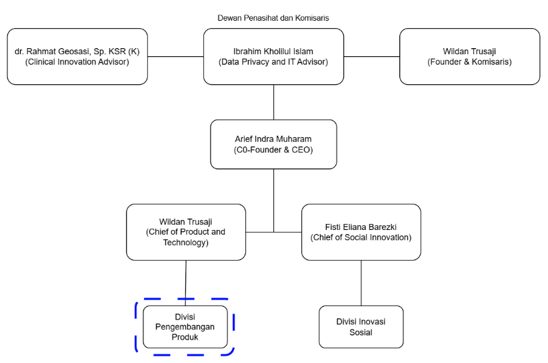
\includegraphics[width=12.36cm]{figure/struktur-organisasi-karla.png}
  \caption{Struktur PT Bangga Teknologi Produktif}
\end{figure}

Pada saat pelaksanaan PKL, tim PKL ditempatkan di Divisi Pengembangan Produk yang berfokus pada penelitian dan pengembangan.

\section{Deskripsi Pekerjaan}
Dalam pelaksanaan Praktek Kerja Lapangan (PKL) yang telah dilaksanakan, penulis bertugas sebagai Backend Engineer yang berfokus pada pengembangan logika sistem, database, dan Dokumentasi API agar decision support system untuk koding dalam klaim BPJS dapat disimulasikan.

Rincian kegiatan yang dilakukan selama periode PKL adalah sebagai berikut.

\noindent\textbf{Fase 1 : Analisis Permasalahan}\\
Dalam fase ini, tim PKL menganalisis dan mencari informasi terkait permasalahan yang diberikan oleh perusahan.

\noindent\textbf{Fase 2 : Analisis Solusi dari Permasalahan}\\
Dalam fase ini, tim PKL menganalisis solusi yang dapat mengatasi permasalahan yang telah disepakati bersama dengan pembimbing lapangan.

\noindent\textbf{Fase 3 : Pengembangan Frontend}\\
Dalam fase ini, penulis mengembangkan backend yang disesuaikan dengan rencana pengembangan sistem.

\noindent\textbf{Fase 4 : Integrasi Frontend Dengan Backend}\\
Dalam fase ini, tim PKL mengintegrasikan Frontend dan Backend yang telah dikembangkan serta memperbaiki kekurangan sistem yang muncul setelah integrasi.

\section{Jadwal Kerja}
\begin{table}[H]
  \centering
  \caption{Jadwal Kerja}
  \begin{tabular}{|l|c|c|c|p{5.5cm}|}
    \hline
    \textbf{Hari} & \textbf{Jam Masuk} & \textbf{Jam Istirahat} & \textbf{Jam Pulang} & \textbf{Keterangan} \\
    \hline
    Senin  & 09.00 & 11.30-13.00 & 17.00 & Kegiatan rutin di Kantor \\ \hline
    Selasa & 09.00 & 11.30-13.00 & 17.00 & Kegiatan rutin di Kantor \\ \hline
    Rabu   & 09.00 & 11.30-13.00 & 17.00 & Kegiatan rutin di Kantor \\ \hline
    Kamis  & 09.00 & 11.30-13.00 & 17.00 & Kegiatan rutin di Kantor, Evaluasi Mingguan \\ \hline
    Jumat  & 09.00 & 11.30-13.00 & 17.00 & Kegiatan rutin di Kantor \\ \hline
  \end{tabular}
\end{table}
